%!TEX root=../document.tex

\section{Ergebnisse}
\label{sec:Ergebnisse}
Für die Umsetzung dieser Übung wurden folgende Technologien verwendet:
Spring-Framework, da es im Vergleich zu anderen Frameworks dieser Art einfach zu verwenden und aufzusetzen ist. Ebenso von Vorteil ist der integrierte Applikationsserver. Die Verwendung von JAX-RS wurde im Rahmen dieser Übung vorgeschrieben. Unser Betreuer gab uns den Hinweis H2, eine dateibasierte und hier leichter zu verwendete Datenbank, statt einer relationalen Datenbank, wie beispielsweise MySQL, zu verwenden. Als Buildmanagement-Tool wurde Maven verwendet, welches bisher wunderbar seine Dienste verrichten konnte. Ein in den Quellen verlinktes Tutorial ('Bootiful' Java EE Support in Spring Boot 1.2) wurde übernommen und entsprechend an die in dieser Übung benötigte Funktionalität angepasst. Wichtige, noch nicht vorhandene Teile waren beispielsweise die RESTful Endpoints für dem Login und die Registrierung, aber auch die Datenbankanbindung mussten angepasst werden. \cite{Bootiful, SpringFramework, JAXRS, Maven, H2}

\subsection{Link zum Repository}
\label{subsec:Link zum Repository}
Die Abgabe wurde, wie üblich, auf GitHub zur Verfügung gestellt. \cite{GitHub-Repo}
\newpage

\section{Akzeptanzkriterien}
\subsection{Registrierung}
Die Überprüfung der Funktionalität gemäß den vorgeschriebenen Anforderungen wurde mittels des Firefox-Plugins \textit{HttpRequester} durchgeführt. \cite{HTTPFirefox}

\subsubsection{Erfolgreiche Registrierung}

Sollten alle Parameter gegeben sein, so wird ein Account erstellt.

\begin{figure}[H]
	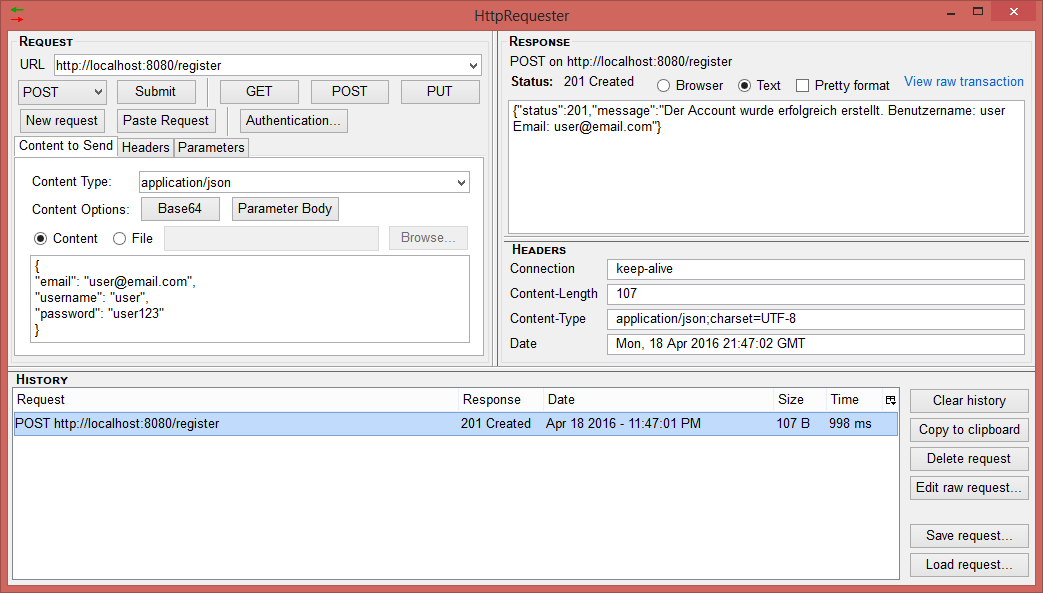
\includegraphics[width=1\textwidth]{images/register_ok.png}
	\caption{Erfolgreiche Registrierung des Benutzers}
\end{figure} 
\clearpage

\subsubsection{Fehlende(r) Parameter}

Sollte ein oder mehrere Parameter fehlen, so wird der Account nicht erstellt. Der Benutzer wird auf seinen Fehler entsprechend hingewiesen.

\begin{figure}[H]
	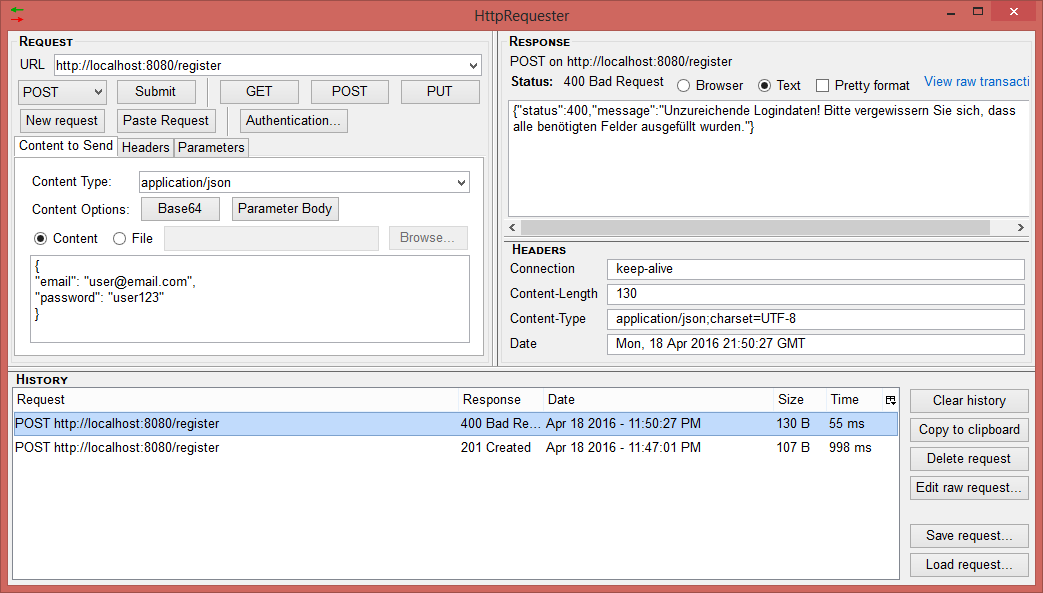
\includegraphics[width=1\textwidth]{images/register_param_missing.png}
	\caption{Eingabe von fehlerhaften Parametern}
\end{figure}
\clearpage

\subsubsection{Bereits vorhandener Benutzer}

Sollte der Benutzer bereits in der Datenbank registriert sein, so wird der Account nicht angelegt. Der Benutzer wird darüber entsprechend informiert.

\begin{figure}[H]
	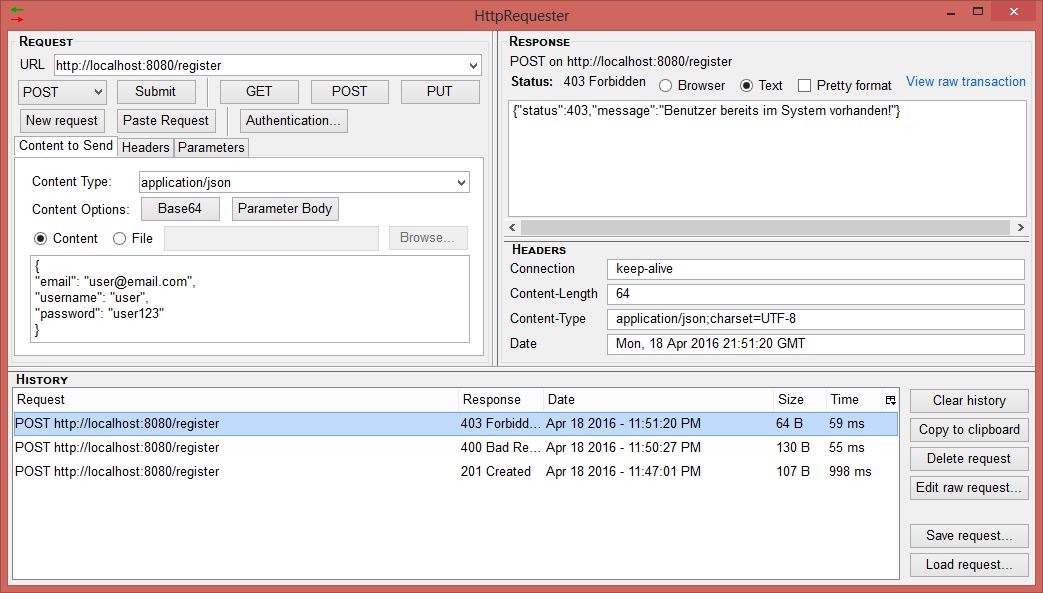
\includegraphics[width=1\textwidth]{images/register_dupl.png}
	\caption{Benachrichtigung über bereits vorhandenen Account}
\end{figure}
\clearpage

\subsection{Login}
\subsubsection{Erfolgreicher Login}

Sollten alle Parameter gegeben und der Benutzer in der Datenbank vorhanden sein, so wird dieser mit Erfolg angemeldet.

\begin{figure}[H]
	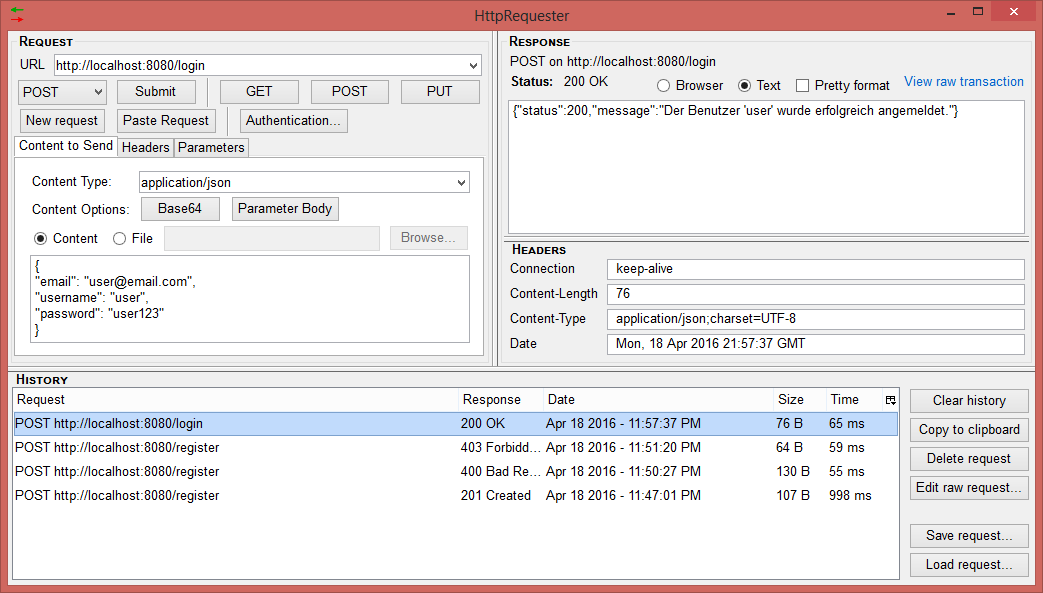
\includegraphics[width=1\textwidth]{images/login_ok.png}
	\caption{Erfolgreicher Login eines Benutzers}
\end{figure}
\clearpage

\subsubsection{Fehlende(r) Parameter}

Sollte ein oder mehrere Parameter beim Loginvorgang fehlen, so wird der Benutzer entsprechend darauf hingewiesen.

\begin{figure}[H]
	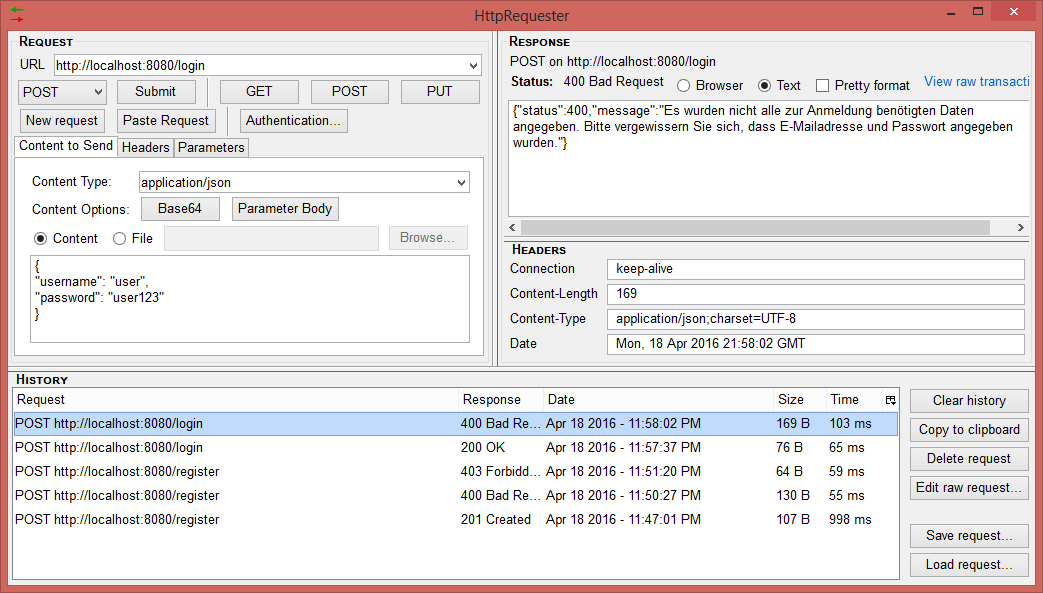
\includegraphics[width=1\textwidth]{images/login_param_missing.png}
	\caption{Benachrichtigung über fehlende Parameter}
\end{figure}
\clearpage

\subsubsection{Benutzer nicht vorhanden}

Sollte der Benutzer nicht in der Datenbank gefunden werden können, so wird dieser entsprechend darauf hingewiesen.

\begin{figure}[H]
	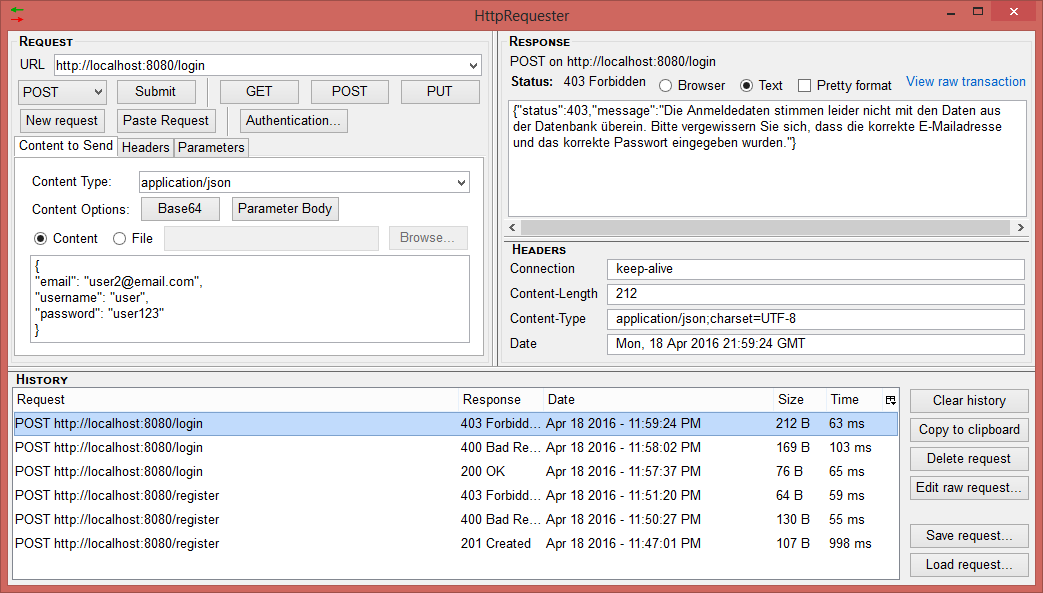
\includegraphics[width=1\textwidth]{images/login_not_registered.png}
	\caption{Nicht vorhandener Benutzer}
\end{figure}

\subsection{Fazit}
Zunächst gab es Probleme mit dem Deployment, welche durch einen Blick auf bestehende Lösungen von anderen Mitschülern und einer kurzen Recherche mithilfe einer Suchmaschine innerhalb von ca. 15 Minuten gelöst werden konnten. Die benötigte Zeit zum Lösen der Aufgabe lag bei ca. 5 Stunden.